\chapter{Pushdown Automata, CFG<-->PDA}

\section{CFG: Context Free Grammars}

Using FA and regular expressions, some language such as \(\{ 0^n1^n | n \geq 0 \} \) can not be described. 

\textbf{Context-free grammars}  is a more powerful method of describing languages. Such grammar can describe certain features that have a recursive structure, which makes them useful in a variety of applications.

An important application of CFG occurs in the specification and compilation of programming languages. A number of methodologies facilitate the construction of a \textbf{parser} once a CFG is available. Some tools even automatically generate the parser from the grammar.

\begin{example}[CFG example]
    The following CFG we call \(G_1\):

    \begin{align*}
        A &\rightarrow 0A1 \\
        A &\rightarrow B \\
        B &\rightarrow \# 
    \end{align*}

    Shorthand:
    \begin{align*}
        A &\rightarrow 0A1 | B \\
        B &\rightarrow \# 
    \end{align*}

    \begin{itemize}
        \item It contains a collection of \textbf{substitution rules}, also called \textbf{productions}. 
        \item Left side: \textbf{variable}, capital letters
        \item Right side: \textbf{terminals}, analogous to the input alphabet and often represented by lowercase letters, numbers or special symbols
        \item In this example, \(G_1\)'s variables are \(A\) and \(B\), its terminals are 0, 1 and \(\#\).   
    \end{itemize}

    Example of using \(G_1\) to generate string \verb|000#111|:
    \[
        A \Rightarrow 0A1 
        \Rightarrow 00A11
        \Rightarrow 000A111 
        \Rightarrow 000B111 
        \Rightarrow 000\#111 
    \] 

    The above information can be shown in a \textbf{parse tree}:

    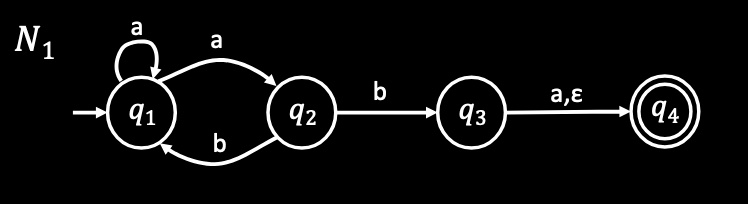
\includegraphics[width=0.8\textwidth]{f2.1.jpg}
\end{example}

\begin{definition}[CFG]
    A \textbf{context-free grammar} is a 4-tuple \((V, \Sigma, R, S)\), where
    \begin{enumerate}
        \item \(V\) is a finite set called the \textbf{variables}
        \item \(\Sigma\) is a finite set, disjoint from \(V\), called the \textbf{terminals}
        \item \(R\) is a finite set of \textbf{rules}, with each rule being a variable and a string of variables and terminals (rule form: \(V \rightarrow (V \cup \Sigma)^*\))
        \item \(S \in V\) is the start variable       
    \end{enumerate}  

    For \(u, v \in (V \cup \Sigma)^*\) write
    \begin{enumerate}
        \item \(u \Rightarrow v\) if can go from \(u\) to \(v\) with one substitution step in \(G\).
        \item \(u \xRightarrow{*} v\) if can go from \(u\) to \(v\) with some number of substitution steps in \(G\). \\
        \(u \Rightarrow u_1 \Rightarrow u_2 \Rightarrow \cdots \Rightarrow u_k = v\) is called a derivation of \(v\) from \(u\).   
    \end{enumerate} 
\end{definition}

\begin{definition}[Context Free Language]
    Given \(L(G) = \{ w|w \in \Sigma^* \; and \; S \xRightarrow{*} w \} \)\\ 
    \(A\) is a \underline{Context Free Language}(CFL) if \(A = L(G)\) for some CFG G.  
\end{definition}

\begin{example}
    We have 2 set of rules here:

    \(C_1\):
    \begin{align*}
        B &\rightarrow 0B1 | \epsilon \\
        B1 &\rightarrow 1B \\
        0B &\rightarrow B0
    \end{align*}

    \(C_2\):
    \begin{align*}
        S &\rightarrow 0S | S1 \\
        R &\rightarrow RR
    \end{align*} 

    \(C_1\) is not a CFG, because the left side is not pure variable, it has "context". 

    \(C_2\), on the other hand, even though we can not derive a string with all terminals, but it does not violate the rule, so \(C_2\) is a CFG. 
\end{example}

\begin{example}[CFG]
    \(G_2\):
    \begin{align*}
        E &\rightarrow E + T | T \\
        T &\rightarrow T \times F | F \\
        F &\rightarrow (E) | a
    \end{align*}  

    \(V = \{ E, T, F \} \) 

    \(\Sigma = \{ +, \times, (, ), a \} \) 

    \(R\) = the 6 rules above 

    \(S = E\) 

    Showing the generating tree, it even shows the precedence of the operator \(\times\) is higher than \(+\):

    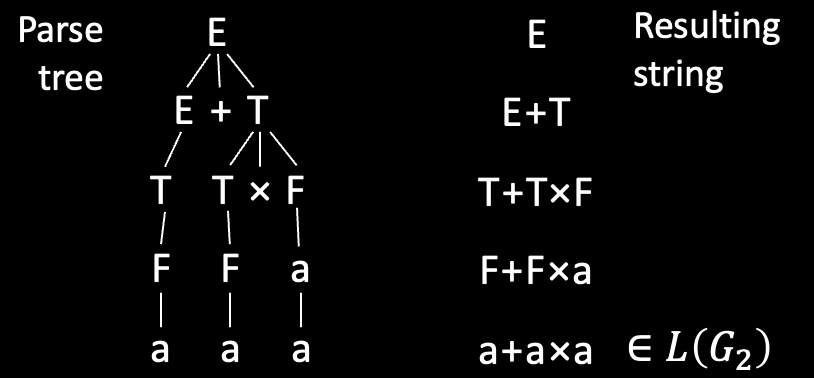
\includegraphics[width=0.6\textwidth]{f4.1.jpg}

    If a string has 2 different parse trees then it is derived \textbf{ambiguously} and we say that the grammar is \underline{ambiguous}.
\end{example}

\begin{example}[Ambiguity]
    \(G_2\):
    \begin{align*}
        E &\rightarrow E + T | T \\
        T &\rightarrow T \times F | F \\
        F &\rightarrow (E) | a
    \end{align*} 

    \(G_3\) 
    \[
        E \rightarrow E +E |E \times E | (E) | a
    \]

    Both of them recognize the same language, \(L(G_2) = L(G_3)\), however \(G_2\) is an unambiguous CFG and \(G_3\) is ambiguous. 

    This tree shows the ambiguity of \(G_3\):
    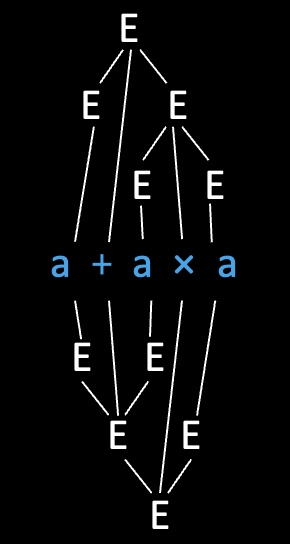
\includegraphics[height=0.2\textheight]{f4.2.jpg} 
\end{example}

\section{Pushdown Automata (PDA)}

The \textbf{Pushdown Automaton} operates like  an NFA except can \underline{write-add}(push) or \underline{read-remove}(pop) symbols from the top of stack.

\begin{figure}[h]
    \centering
    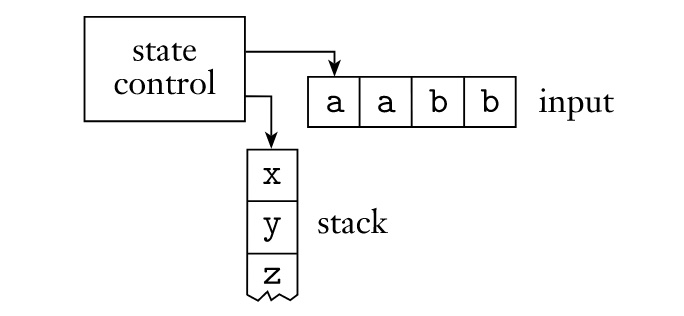
\includegraphics[width=0.6\textwidth]{f2.12.jpg}
    \caption{Schematic of a pushdown automaton}
\end{figure}

\begin{example}[PDA]
   PDA for \(D = \{ 0^k1^k|k \geq 0 \} \)  

    \begin{enumerate}
        \item Read 0s from input, push onto stack until read 1.
        \item Read 1s from input, while popping 0s from stack
        \item Enter accept state if stack is empty (acceptance only at end of input)
    \end{enumerate}
\end{example}

\begin{definition}[PDA]
    A \textbf{pushdown automaton} is a 6-tuple \((Q, \Sigma, \Gamma, \delta, q_0, F)\), where \(Q, \Sigma, \Gamma, F \) are all finite sets:
    \begin{enumerate}
        \item \(\Sigma\) input alphabet 
        \item \(\Gamma\) stack alphabet
        \item \(\delta\): \(Q \times \Sigma_\epsilon \times \Gamma_\epsilon \rightarrow \P(Q \times \Gamma_\epsilon)\) (\(\Sigma_\epsilon = \Sigma \cup \{\epsilon\}\) and \(\Gamma_\epsilon = \Gamma \cup \{ \epsilon \} \), we allow nondeterminism here)\\  
        Left side is the domain(the set of possible inputs to a function) of the transition function; The current state, and the reading(popping) from the top of the stack and reading from the input (can read \(\epsilon\)) decide the input of the transition function \\
        Right side is the writing, the combination of the state and the writing to the top of the stack (can write \(\epsilon\)) decide the output of the transition \\
        \item \(q_0\): the start state
        \item \(F\): the accept states  
    \end{enumerate}
    

    For a transition function like \(\delta(q, a, c) = \{(r_1, d), (r_2, e)\} \), the current state is \(q\), and reading an input \(a\) and popping from the stack \(c\), then we might end up going to:
    \begin{itemize}
        \item state \(r_1\) and writing \(d\)  to the top of stack
        \item state \(r_2\) and writing \(e\)  to the top of the stack 
    \end{itemize} 
\end{definition}

One interesting thing about this definition is that we have no primitive to decide whether the stack is empty at the end.

The reason for that is \textbf{we don't need to}! Because we can write special symbol to the bottom of the stack at the beginning when the machine starts.

\begin{remark}
    Should do some example here to understand deeper into the PDA.   
\end{remark}

\begin{theorem}[Converting CFGs to PDAs]
    If \(A\)  is a CFL then some PDA recognizes \(A\). 
\end{theorem}
